\documentclass[main.tex]{subfiles} % Subfile-Class


% ============================================================================== %
%                            Subfile document                                    %
% ============================================================================== %

\begin{document}

% Template

\subsubsection{Greifeinheit}


Die Abbildung~\ref{fig:Greifereinheit} veranschaulicht das Greiferkonzept des Roboters. Dieses Konzept wurde basierend auf der Evaluierung 
im Anhang~\ref{appendix:Greifereinheit} weiterentwickelt. Im folgenden Abschnitt wird die Funktionsweise des Greifers im Detail beschrieben.

\begin{figure}[H]
    \centering
    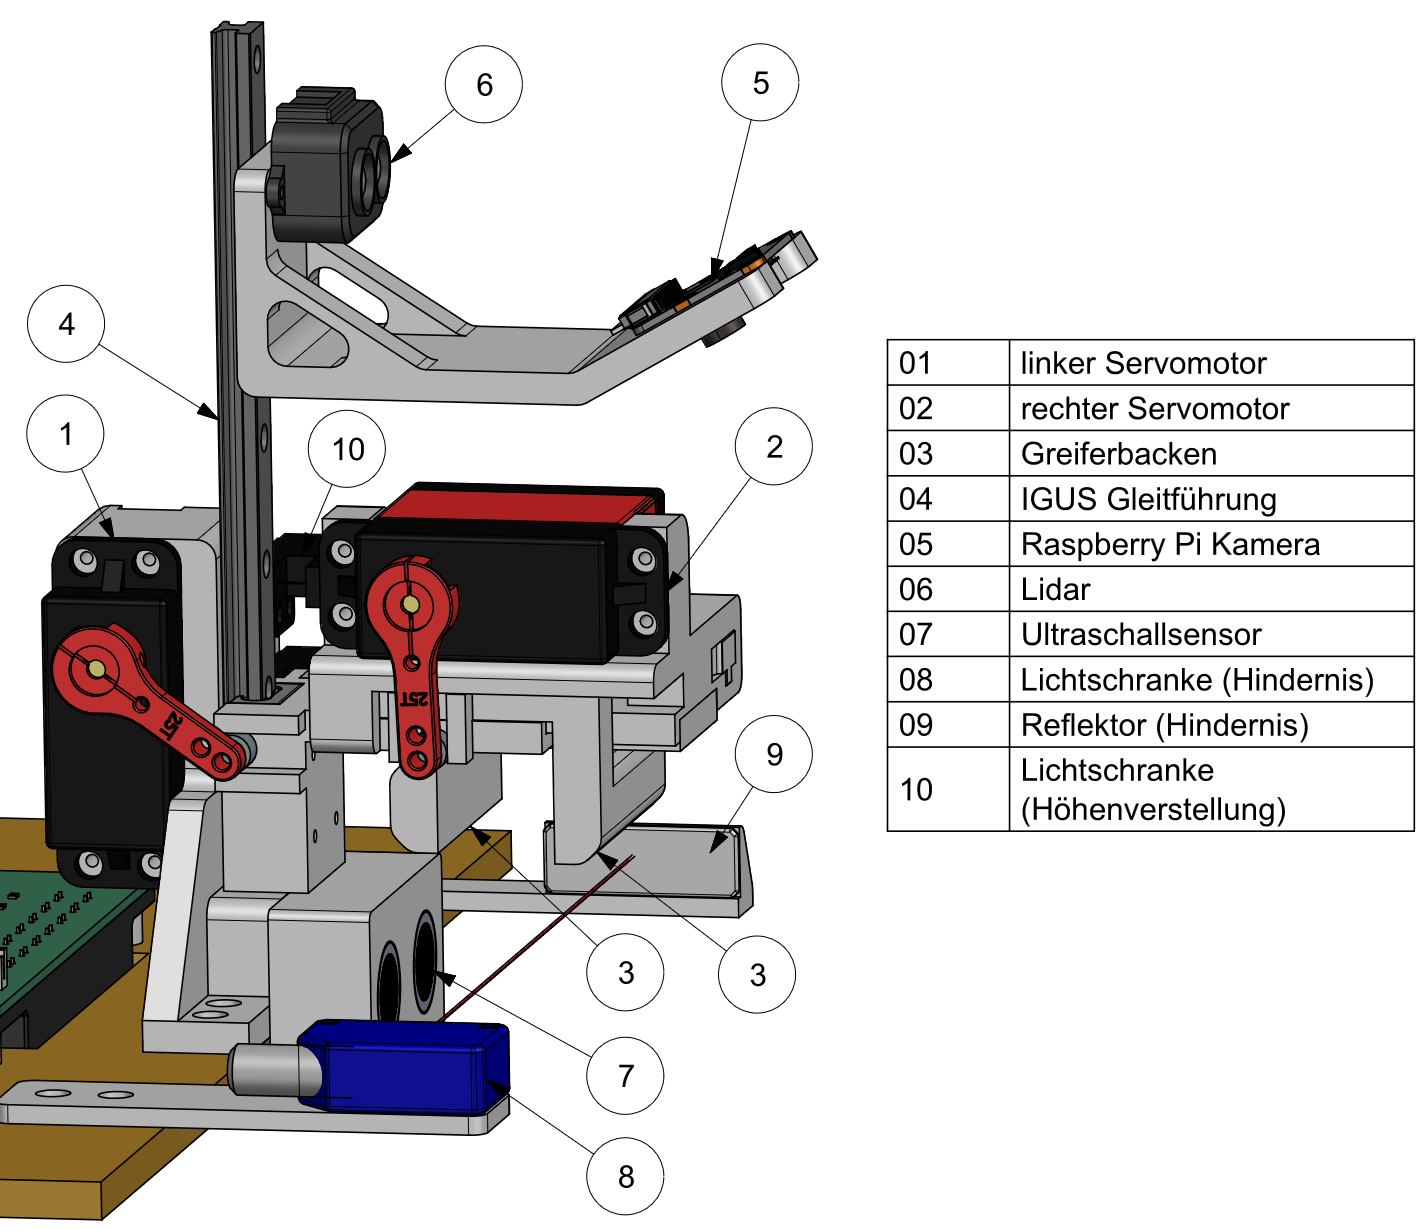
\includegraphics[width=1\textwidth]{Greifereinheit_Uebersicht.png}
    \caption{Übersicht der Greifereinheit im NX Siemens}~\label{fig:Greifereinheit}
\end{figure}

Der Greifer verfügt über zwei Backen, die parallel zueinander verschoben werden, um das Hindernis sicher zu greifen. 
Dieser Vorgang wird von einem Servomotor gesteuert. Konkret bewegt der Hebel vom Servomotor eine der beiden Backen horizontal. 
Diese Backe ist mit einer Zahnstange ausgestattet, die ein innenliegendes Zahnrad antreibt. Das Zahnrad überträgt die 
Bewegung auf die gegenüberliegende Backe, sodass sich beide Backen synchron, aber in entgegengesetzter Richtung bewegen. 
Die Höhenverstellung ist ebenfalls mit einem Servomotor gelöst.Dieser bewegt den Greifer entlang einer Gleitführung von IGUS 
nach oben und unten. Die benötigten Drehmomente für den Servomotor befinden sich im Anhang~\ref{appendix:Greifereinheit}.

\newpage

Die Abbildung~\ref{fig:Greiferablauf} zeigt den Ablauf des Greifvorgangs in mehreren Bildern. Die Bewegung des Motors werden mit einem gelben Pfeil dargestellt:

\paragraph{Positionierung der Greifeinheit} 
Von Position 1 zu 2 dreht der linke Servomotor die Greifeinheit entlang einer Gleitführung nach unten, nachdem ein Hindernis erkannt wurde.

\paragraph{Greifen des Hindernisses} 

Von Position 2 zu 3 bewegt der rechte Servomotor die Backen horizontal, wodurch sich beide Backen parallel schliessen und das Hindernis greifen.

\paragraph{Anheben des Hindernisses} 

Von Position 3 zu 4 dreht der linke Servomotor die Greifeinheit leicht nach oben, sodass das Hindernis vom Boden angehoben wird. 
Dadurch wird ein sicherer Transport des Hindernisses gewährleistet.

\begin{figure}[H]
    \centering
    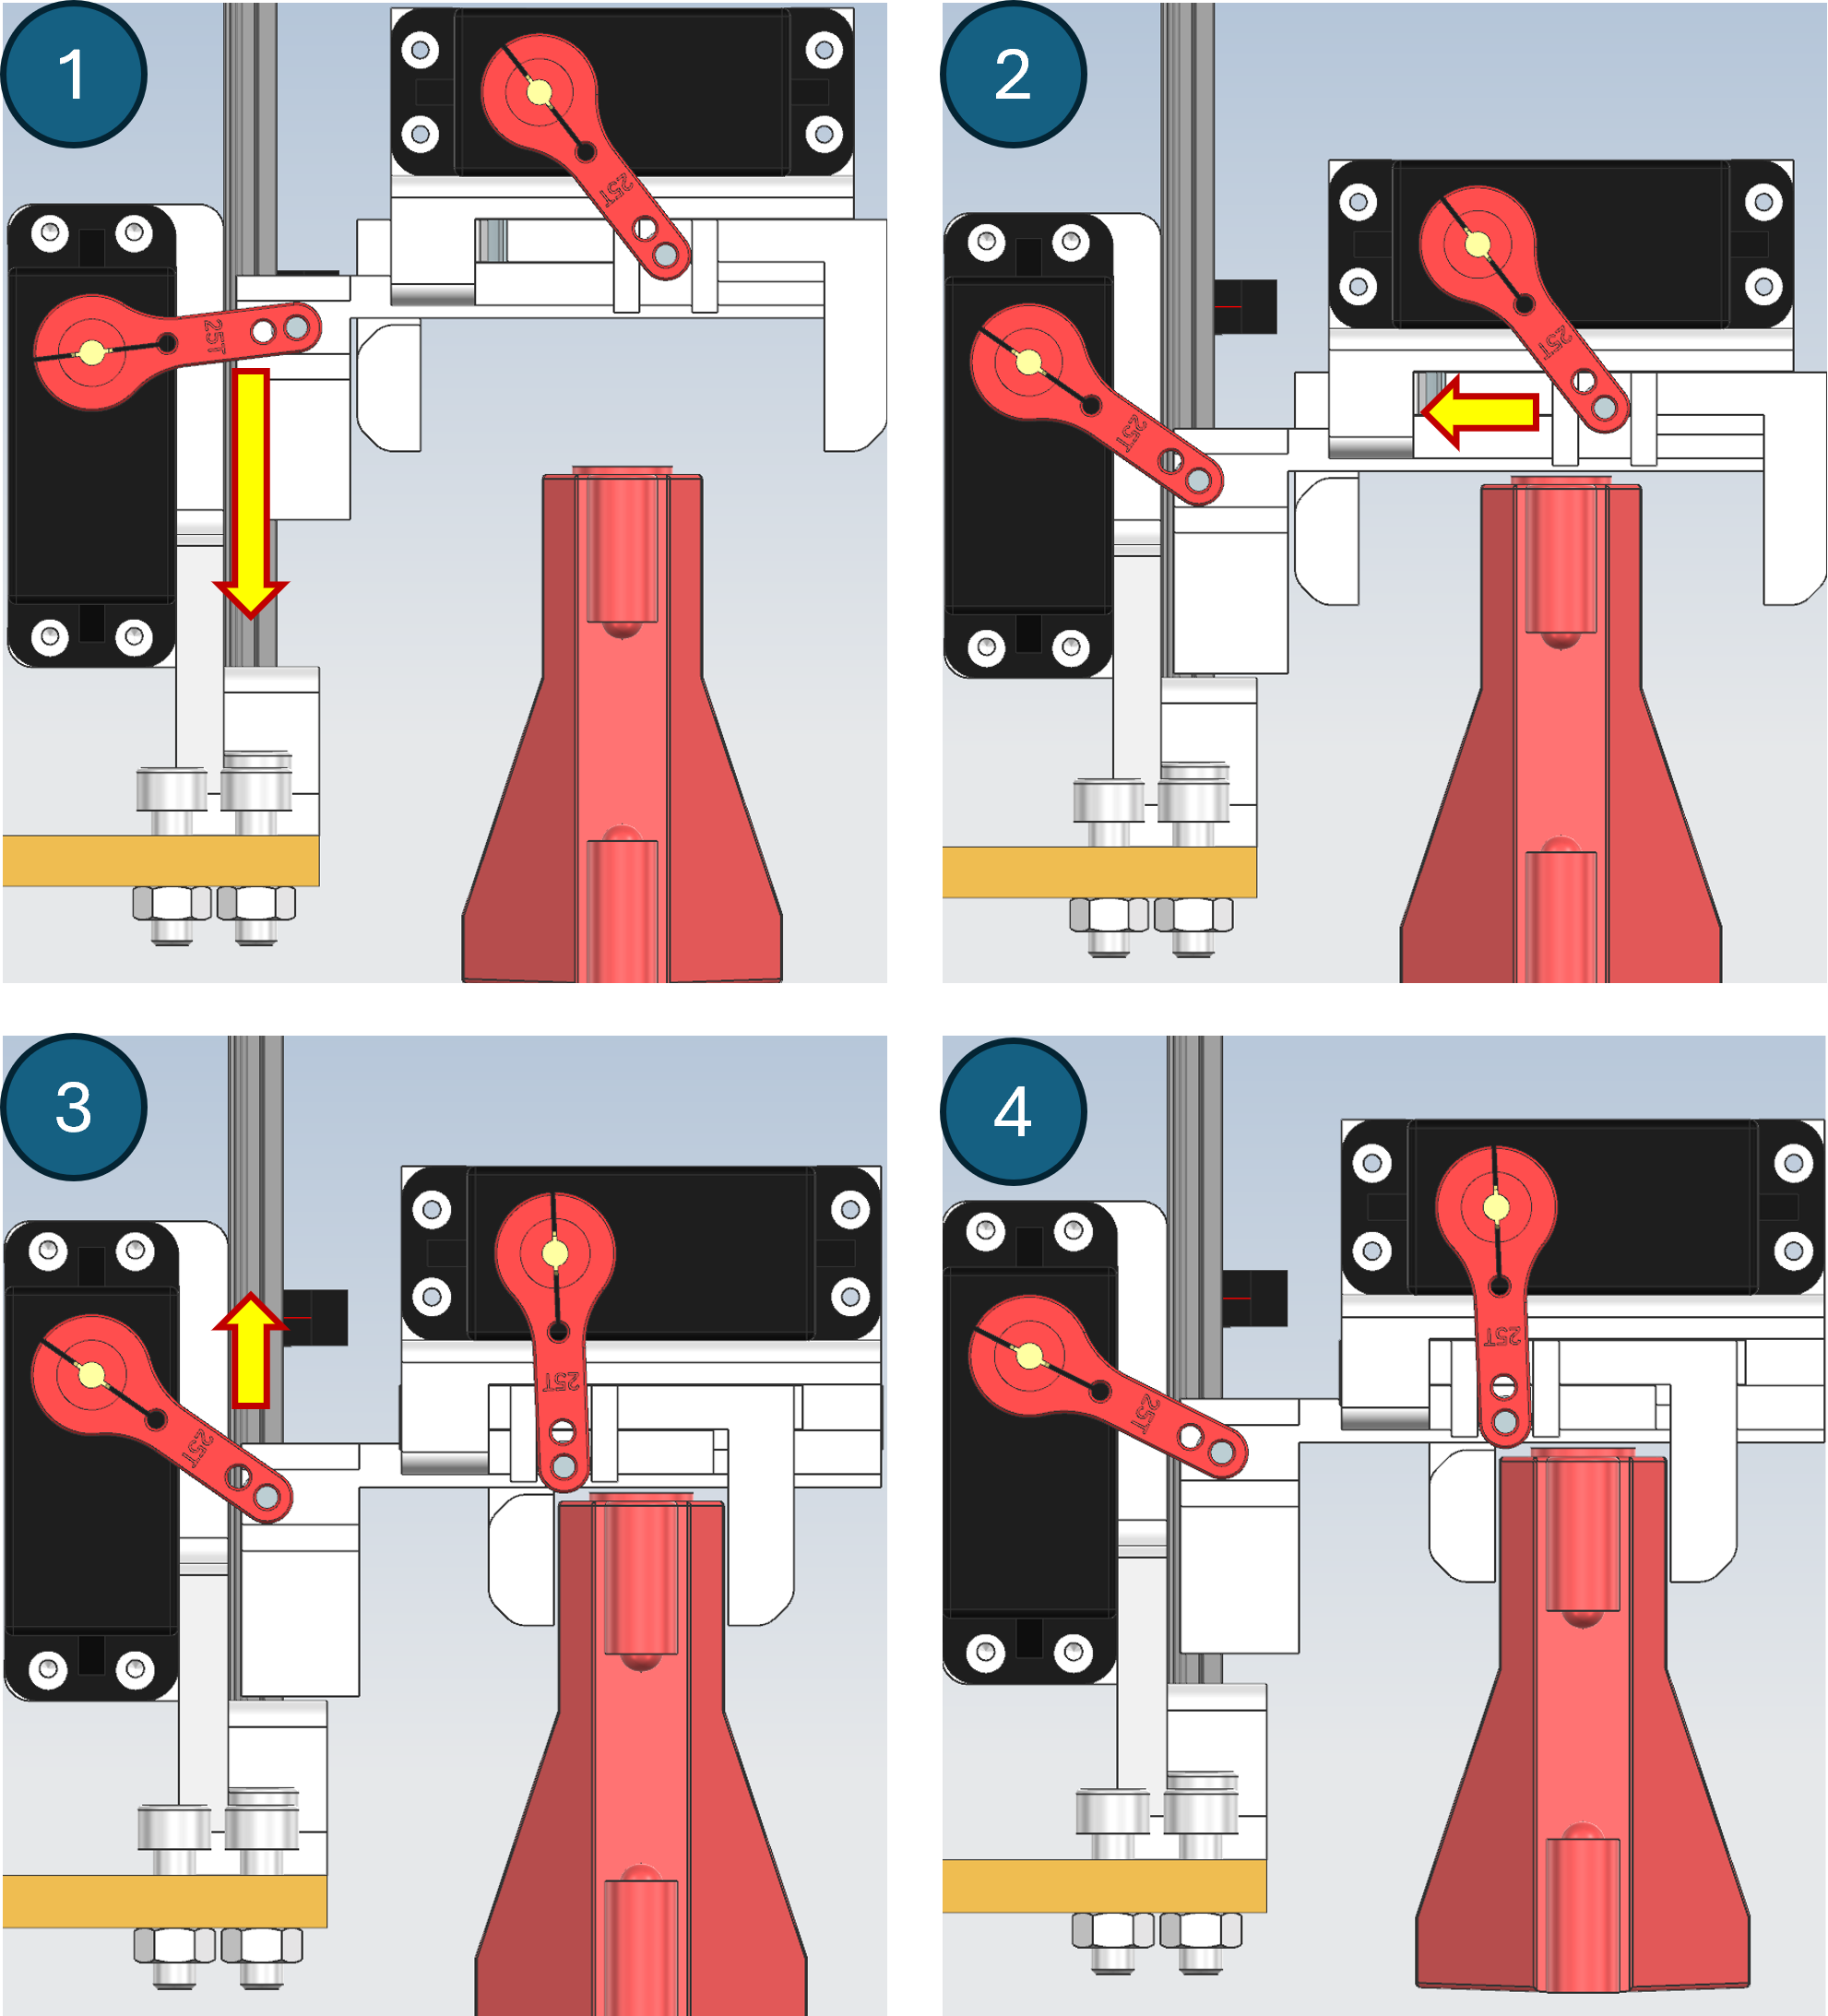
\includegraphics[width=0.85\textwidth]{Greiferablauf.png}
    \caption{Greiferablauf - Anheben des Hindernis}~\label{fig:Greiferablauf}
\end{figure}


\newpage

Die folgende Abbildung~\ref{fig:Greiferprototyp} zeigt einen funktionierenden Greiferprototyp 
aus einer vorherigen Iteration.

\begin{figure}[H]
    \centering
    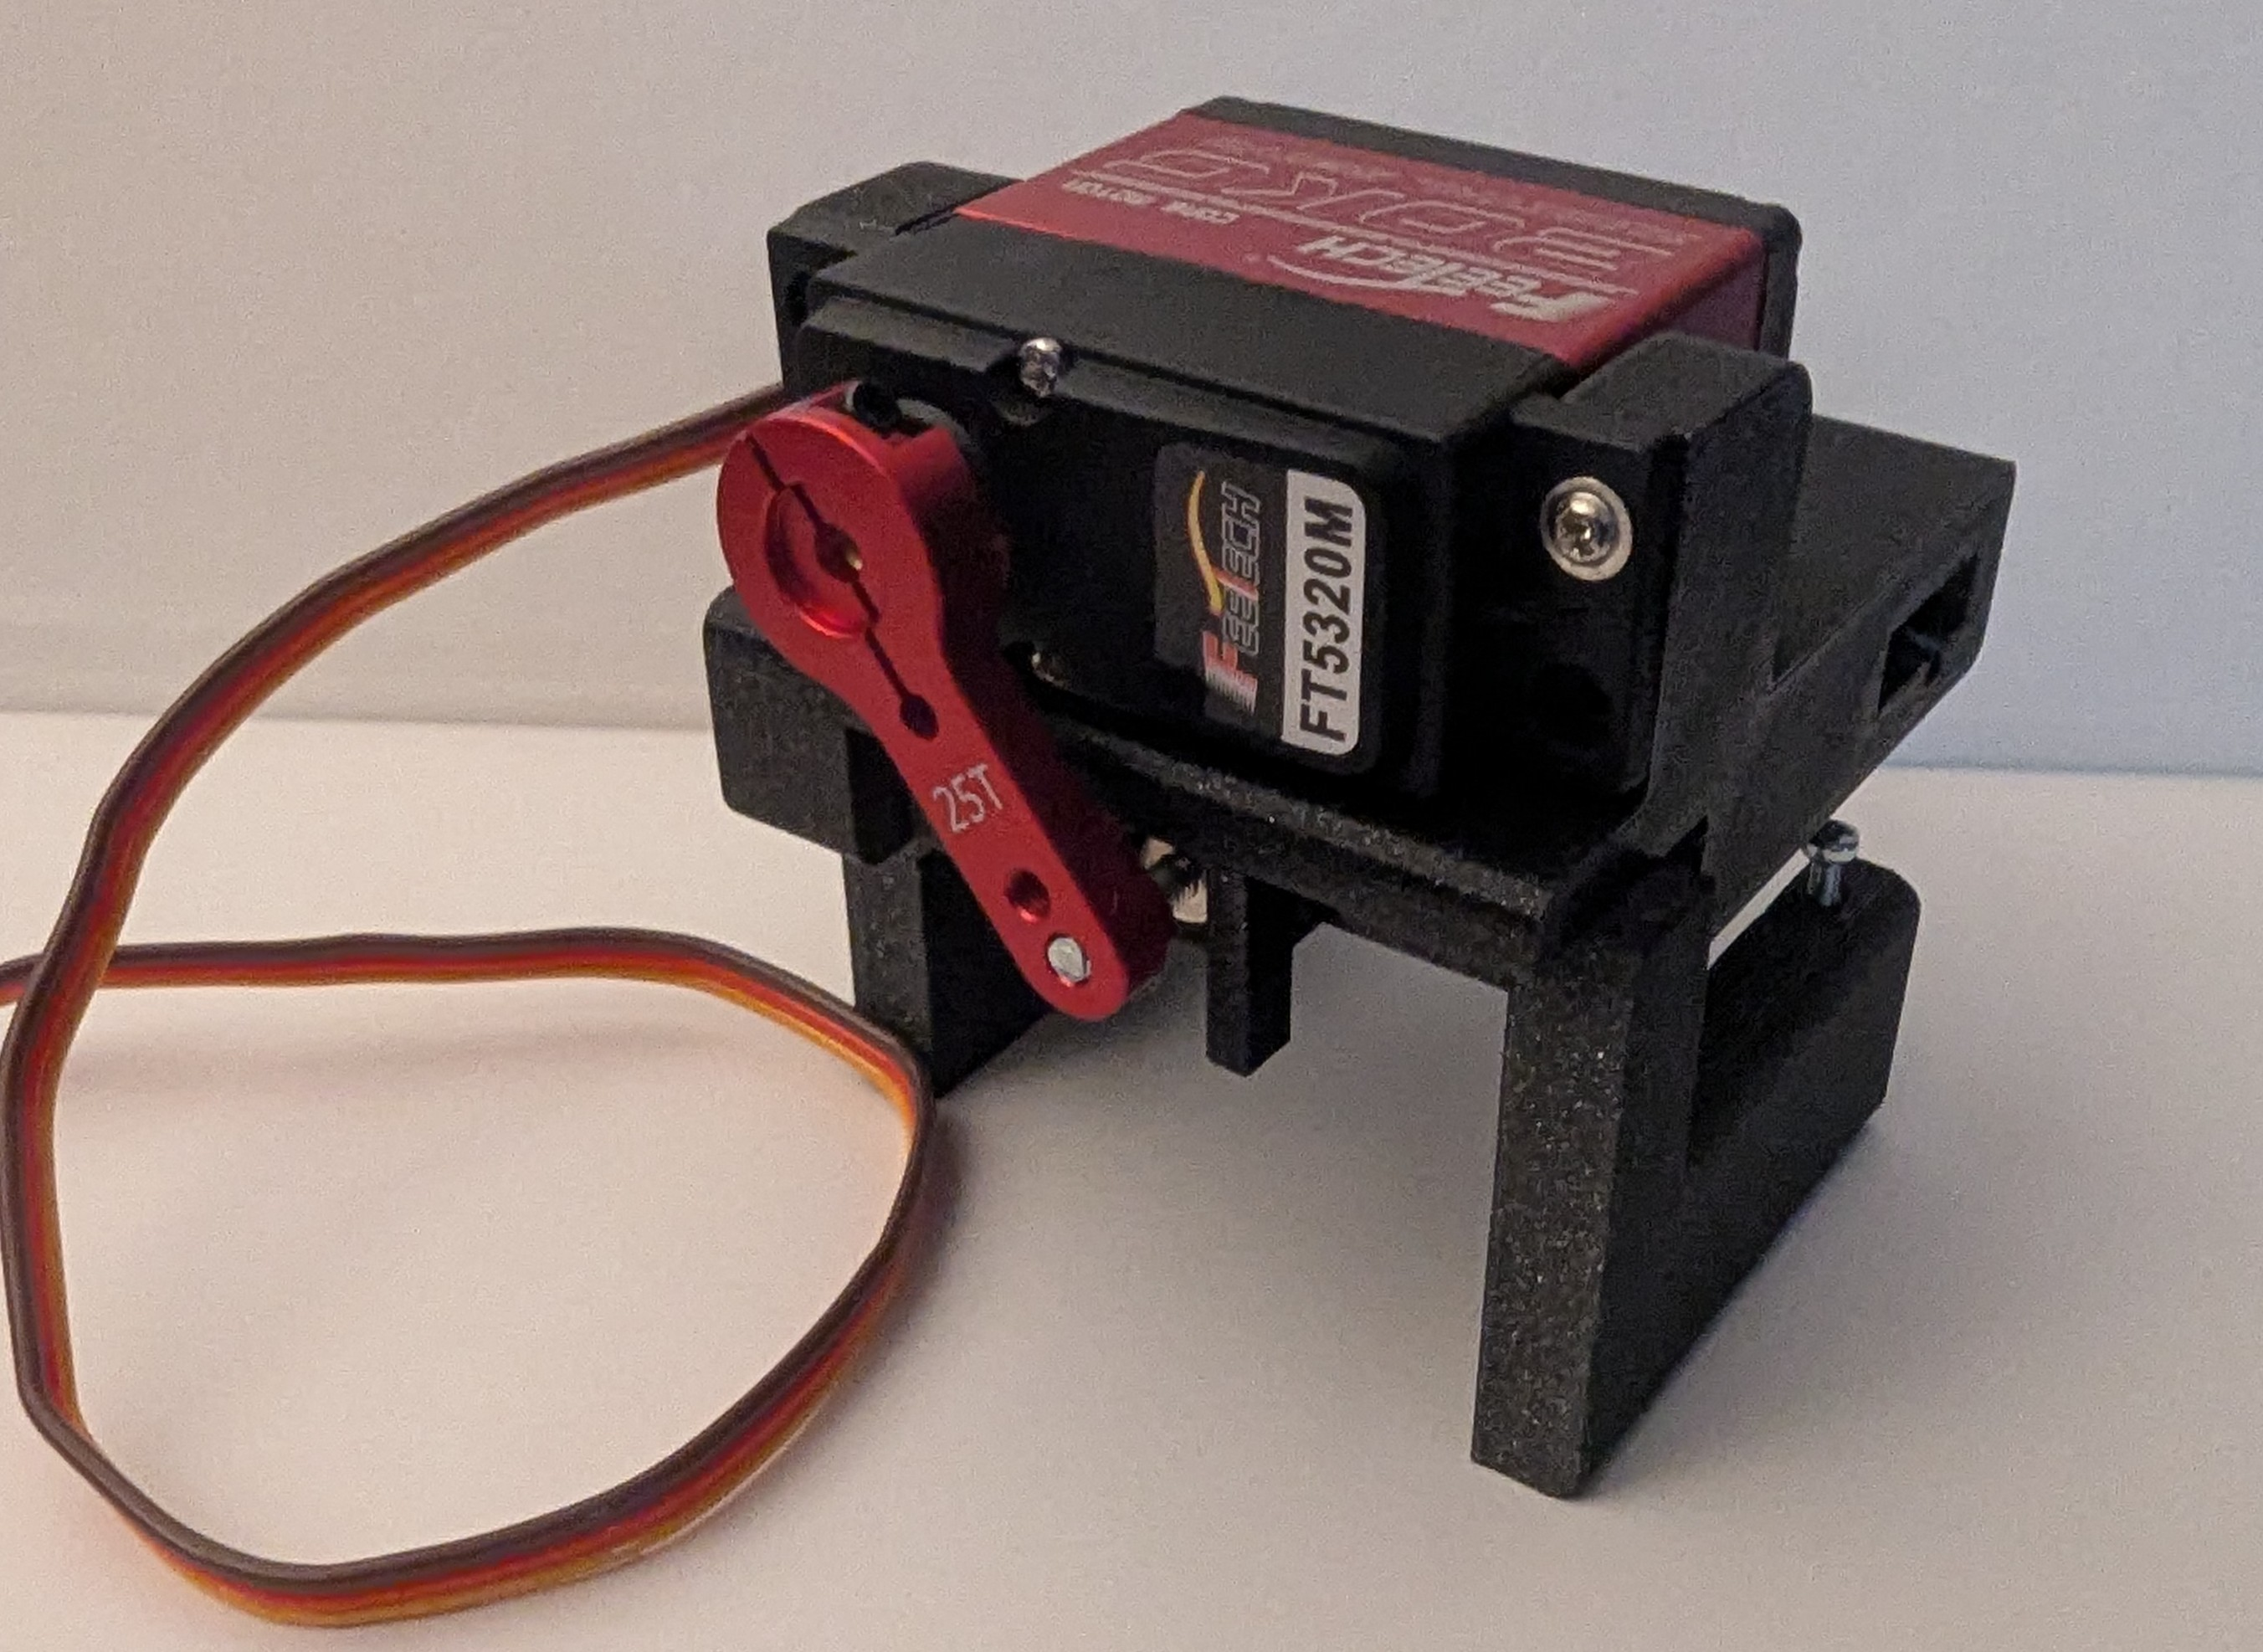
\includegraphics[width=0.75\textwidth]{Greiferprototyp.jpg}
    \caption{Greiferprototyp}~\label{fig:Greiferprototyp}
\end{figure}

\subsubsection*{Sensorikplatzierung}

In diesem Abschnitt werden die verschiedenen Sensoren an der Greifereinheit beschrieben.

\paragraph{Raspberry Pi Kamera - Knotenpunkt}
Die Raspberry Pi Kamera ist auf Höhe 130 mm in einem Winkel von 30° montiert.
In dieser Position kann sie Objekte mit einem Durchmesser von circa 260 mm auf dem Boden erkennen.
Dadurch wird sichergestellt, dass die 120 mm grossen Knotenpunkte sowie die zugehörigen
Knotenabgänge erfasst werden.


\paragraph{Ultraschallsensor und Lichtschranke - Hinderniss}
Der Ultraschallesnor ist auf Höhe 25 mm montiert. Er erkennt Hindernisse frühzeitig,
um Kollisionen mit dem Roboter zu vermeiden. Er sorgt zusätzlich dafür, dass der Roboter an der richtigen 
Position stoppt, um das Hindernis anzuheben. Falls die Positionserkennung für das Greifen 
des Hindernisses im PREN 2 ungenau ist, wird eine weitere Lichtschranke eingesetzt.
Die genaue Funktionsweise wird im Kapitel~\ref{appendix:Abstandssensoren_Kapitel} ausführlicher erklärt.

\paragraph{Lidar - Pylon}
Der Lidar ist in einer Höhe von 150 mm montiert, wodurch er bis zu einer Entfernung
von 2 Metern einen Pylon erkennen kann. Diese Höhe wird benötigt, sodass die Streuung des Lidars auf 2 Metern keinen
Hindernis erfasst. Die genaue Funktionsweise wird im Kapitel~\ref{appendix:Abstandssensoren_Kapitel} ausführlicher erklärt.

\paragraph{Lichtschranke - Höhenverstellung des Greifers}

Die Lichtschranke sind an den Enpositionen der Höhenverstellung montiert.
Sie stellen sicher, dass die Greifer die richtige Höhe erreicht und verhindern
ein Überdrehen des Servomotors, um Beschädigungen an den Komponenten zu vermeiden.

\end{document}
